\section{Theory and Engineering practices}
Detta kapitel listar och i viss mån beskriver teorier och ingenjörspraxis som använts
i undersökningen. Det finns två underkapitel, litteraturstudie och förstudie.

\subsection{Litteraturstudie.}
I detta kapitel anges litteratur och andra källor som har använts för att hitta ingångar
och möjligheter i undersökningen. Förutom de källor som anges finns förmodligen andra 
och kanske bättre källor som denna studie inte använt sig av.

Undersökningen görs utifrån övergripande projektmetoder men också utifrån specifika metoder
och arbetssätt som används av olika kompetenser i projektets team. Vilka dessa kompetenser
är framgår av texten nedan.

\textbf{Övergripande källor}
\begin{itemize}
    \item Projektets hälsa och status
    \item Scrum
    \item Fasindelning
    \item Projektgrunder
    \item Person och gruppdynamik
\end{itemize}

\textbf{Kundrepresentant} - kompetens enligt [Essence 1.0]
\begin{itemize}
    \item Vision
    \item Kravspecifikation
    \begin{itemize}
        \item "Stories
        \item "UseCase"
    \end{itemize}
\end{itemize}

\textbf{Analytiker} - kompetens enligt ...
\begin{itemize}
    \item Arkitektur (Kruchten, 1995)
\end{itemize}

\textbf{Utvecklare} - kompetens enligt ...
\begin{itemize}
    \item Designplan
\end{itemize}

\textbf{Testare} - kompetens enligt ...
\begin{itemize}
    \item Testplan
\end{itemize}

\textbf{Ledning och styrning} - kompetens enligt ...
\begin{itemize}
    \item Projektplanering
    \begin{itemize}
        \item Projektdefinitionen
    \end{itemize}
\end{itemize}

\textit{\textbf{Miljö, hållbar utveckling, etik och jämställdhet}}

\textit{\textbf{Arbetsmiljö}}

\subsection{Förstudie}
Vilka möjligheter till ansats har beaktats och prövats? Brett perspektiv.
Enligt undersökningsstrategin så skall någon projektmetod prövas i ett 
praktiskt projekt och utifrån de erfarenheter som fås görs en värdering
av använda metoder. Frågan är då vilken ansats av projektmetod som skall 
användas. Eftersom erfarenheten av projektarbete hos studenterna i denna 
kurs är liten så fanns det ett färdigt förslag till ansats av projektmetod. 
Detta projektmetodförslag kan senare modifieras av projektgruppen.
Tidigare kursomgångar och lärarens förslag har mynnat ut i följande ansats.
Projektmetoden framgår med god tydlighet av de arbetstavlor som definierats 
i ansatsen, se figurer och bilder.
Vision, projektdefinition, iterativt, Scrum ….
Resultatet av förstudien är att metoderna, som anges i följande kapitel,
har valts för undersökningens genomförande.\\

\begin{enumerate}
    \item \textit{Arbetstavla}
    \begin{figure}[htbp]
        \centerline{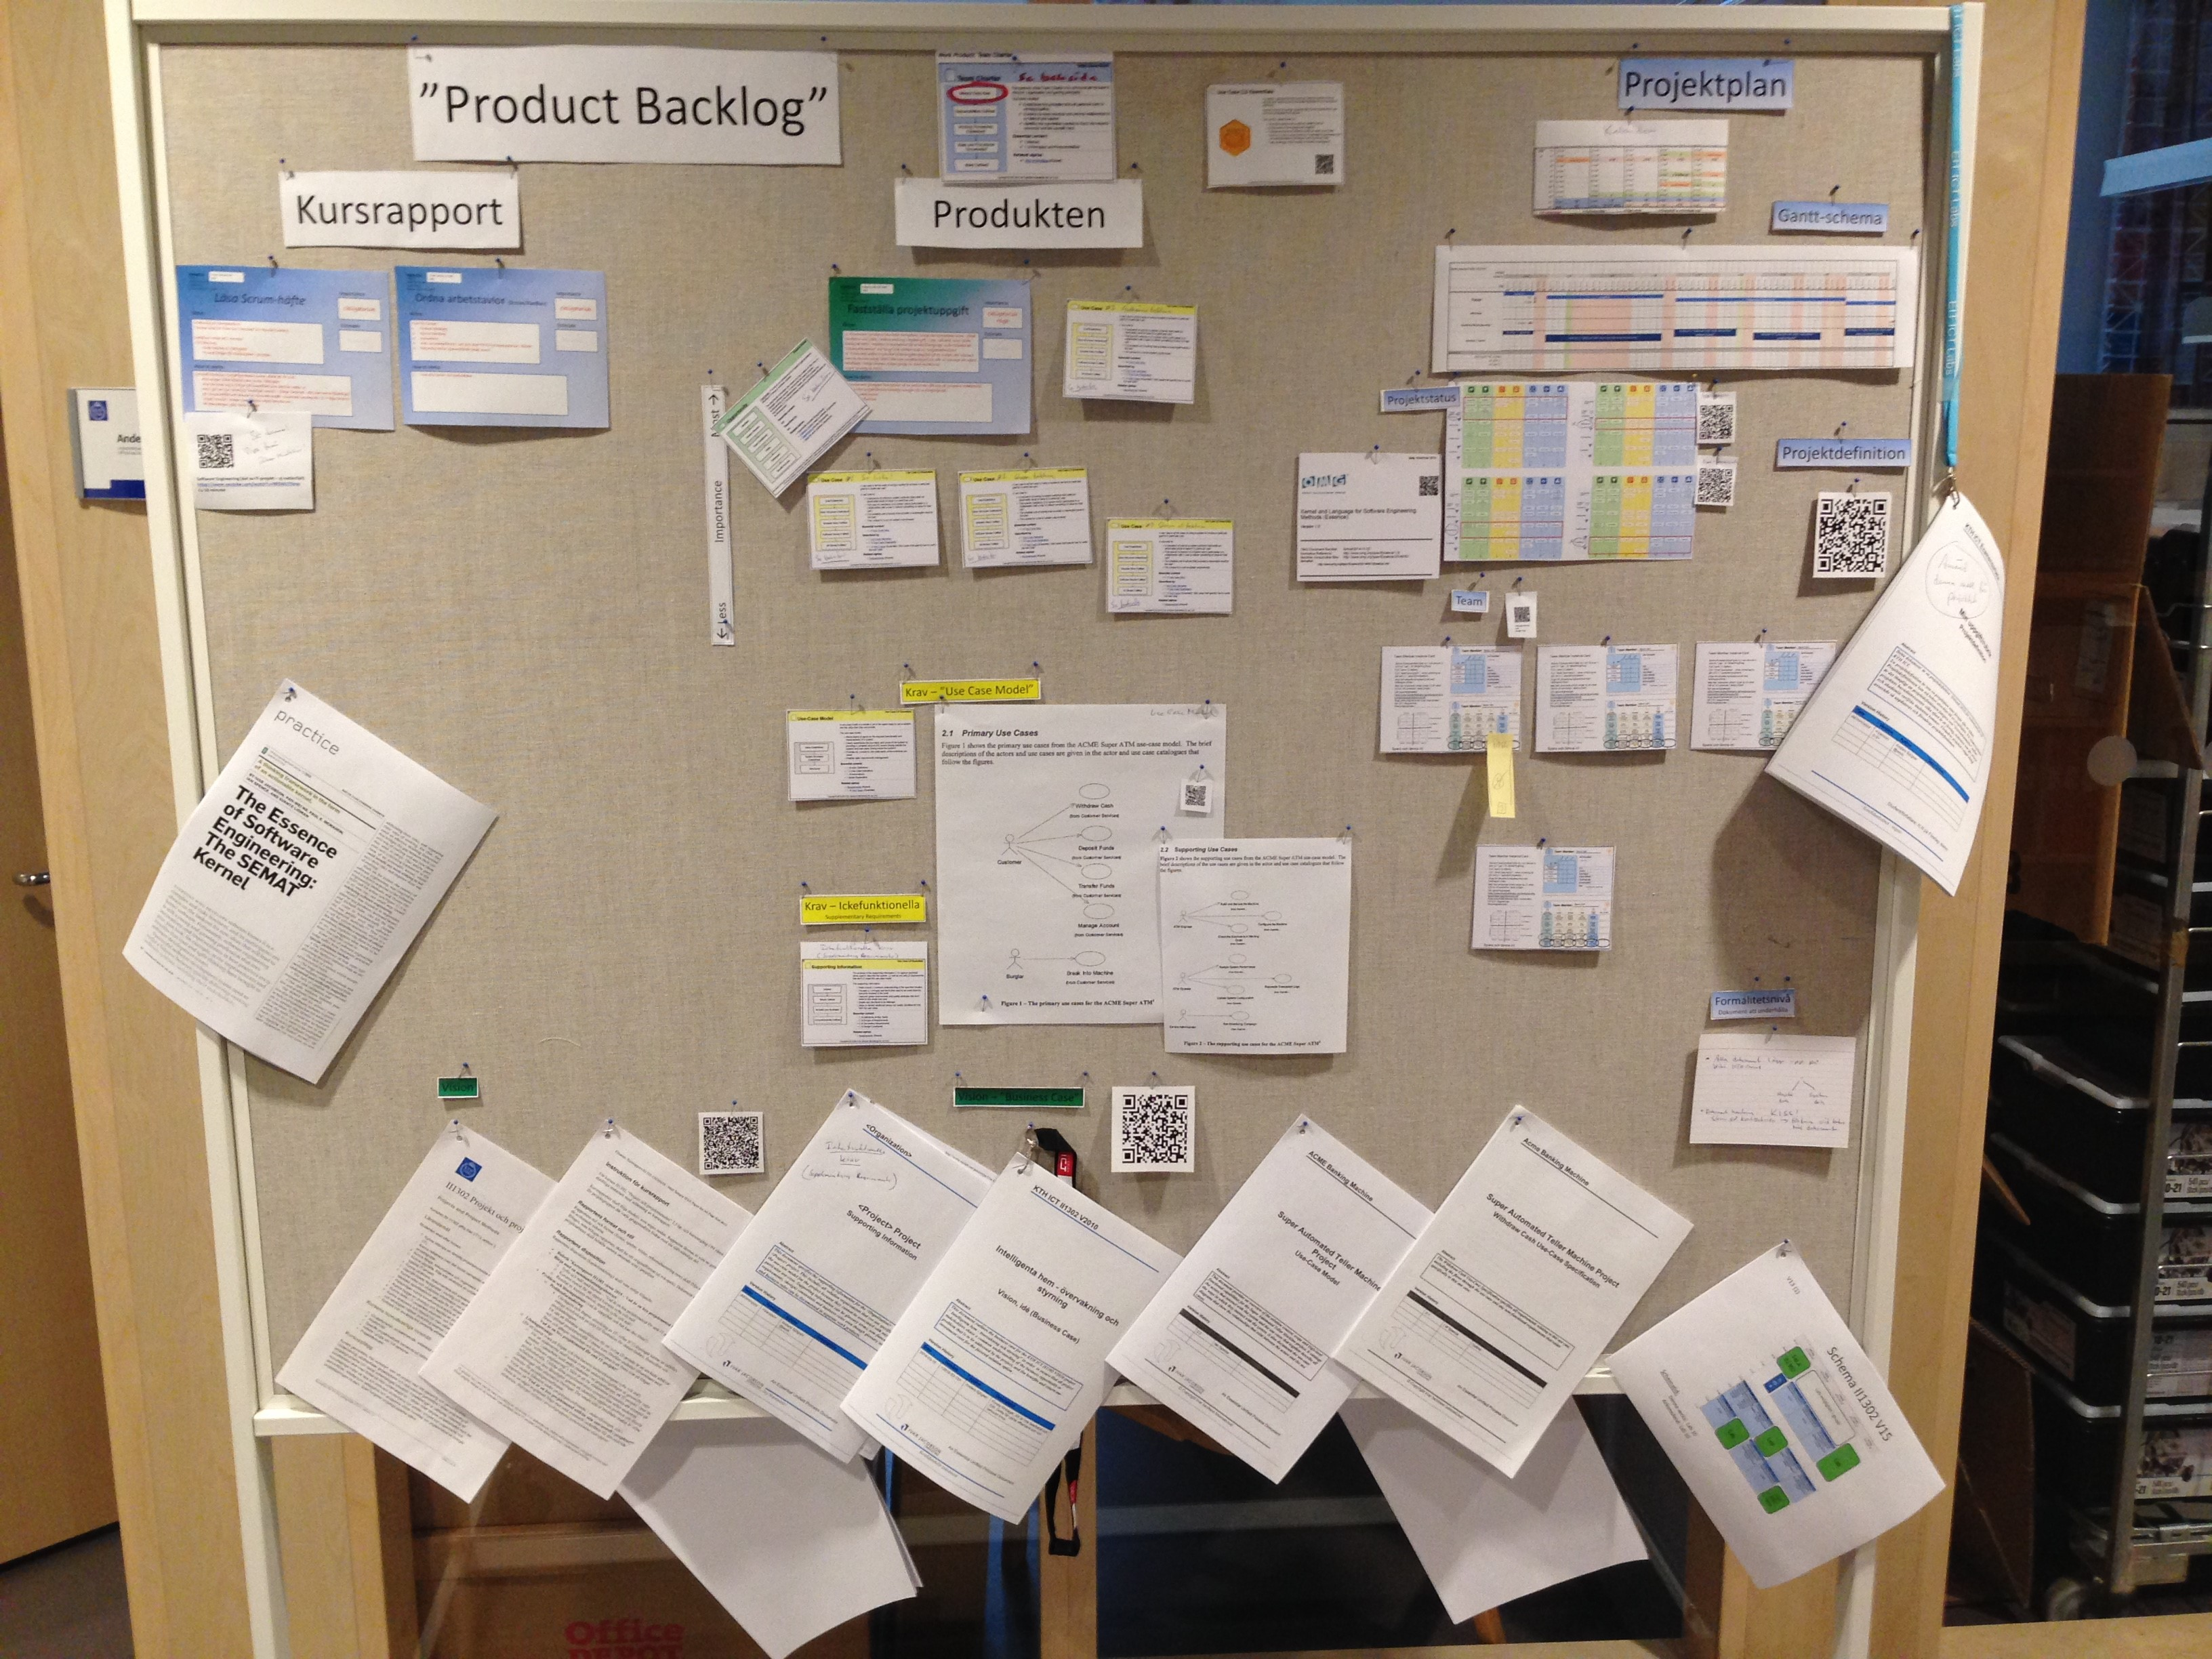
\includegraphics[max height=250px, max width=250px]{Z. images/arbetstavla.jpg}}
        \caption{Arbetstavla "nåldyna"}
        \label{fig}
    \end{figure}
    
    \begin{figure}[htbp]
        \centerline{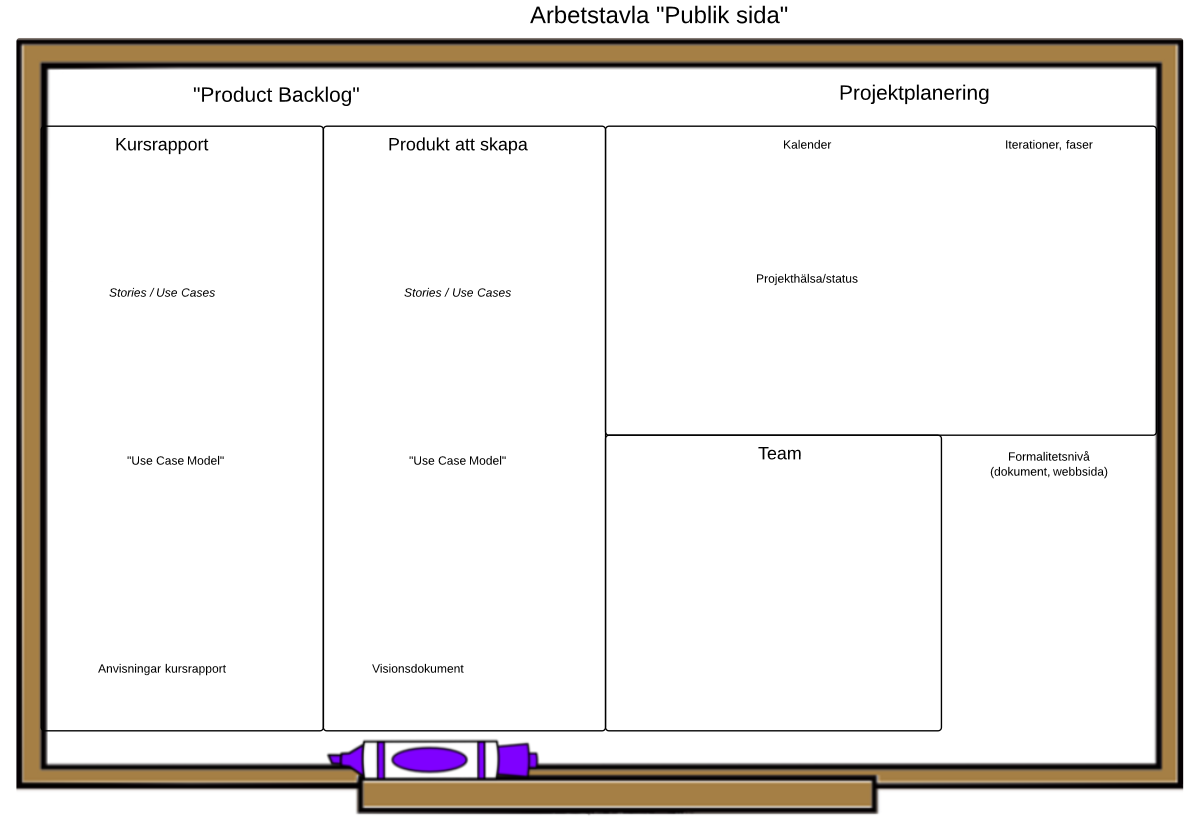
\includegraphics[max height=250px, max width=250px]{Z. images/lucidtavla.png}}
        \caption{Arbetstavla "whiteboard" "Publik sida"}
        \label{fig}
    \end{figure}

    \begin{figure}[htbp]
        \centerline{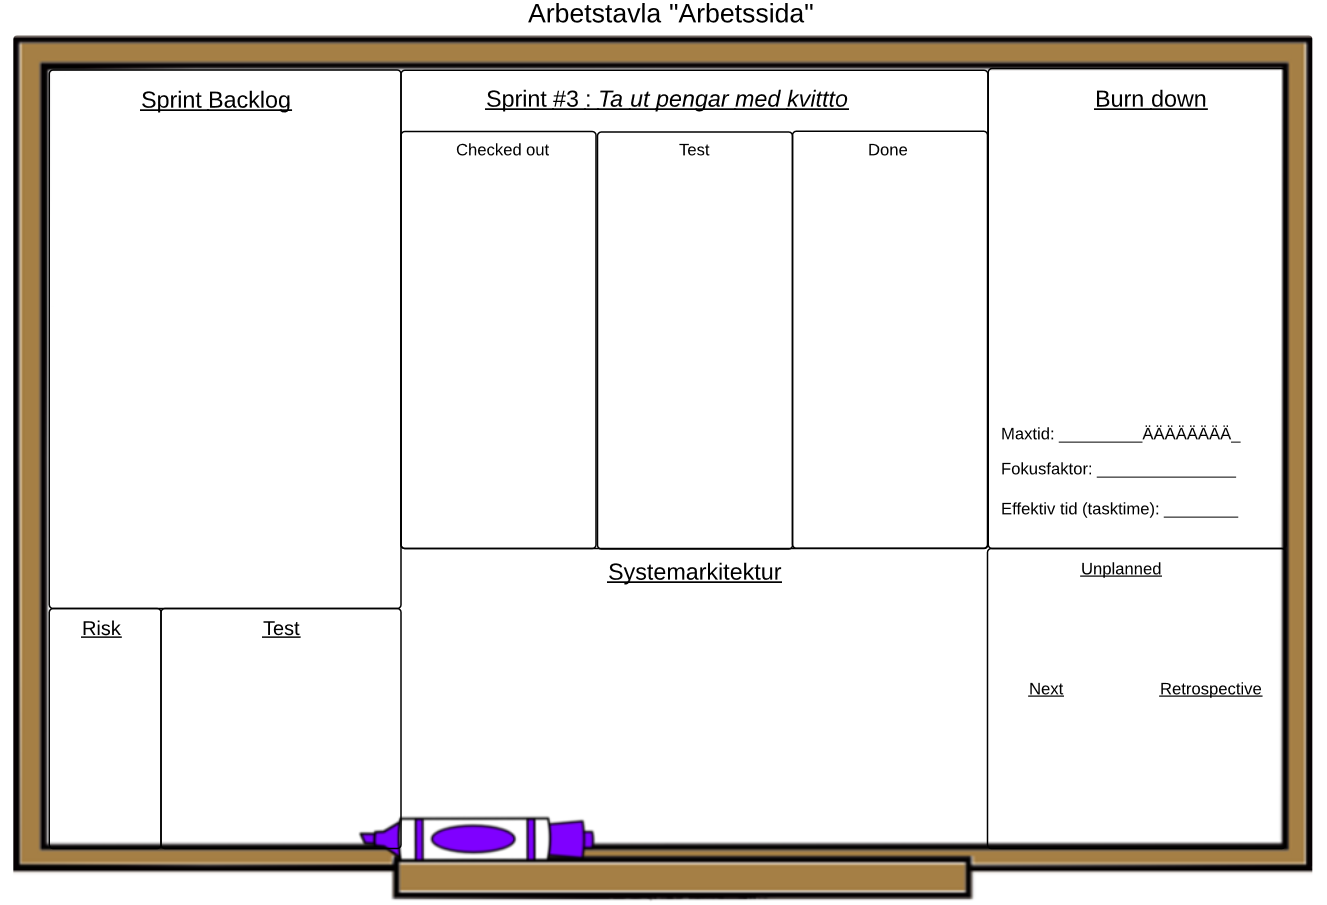
\includegraphics[max height=250px, max width=250px]{Z. images/lucidbaksida.png}}
        \caption{Arbetstavla "whiteboard" "Arbetssida"}
        \label{fig}
    \end{figure}
    \item \textit{Scruminspirerade projektaktiviteter}
    Bilden nedan visar projektmodellens aktiviteter och ordning.

    \begin{figure}[htbp]
        \centerline{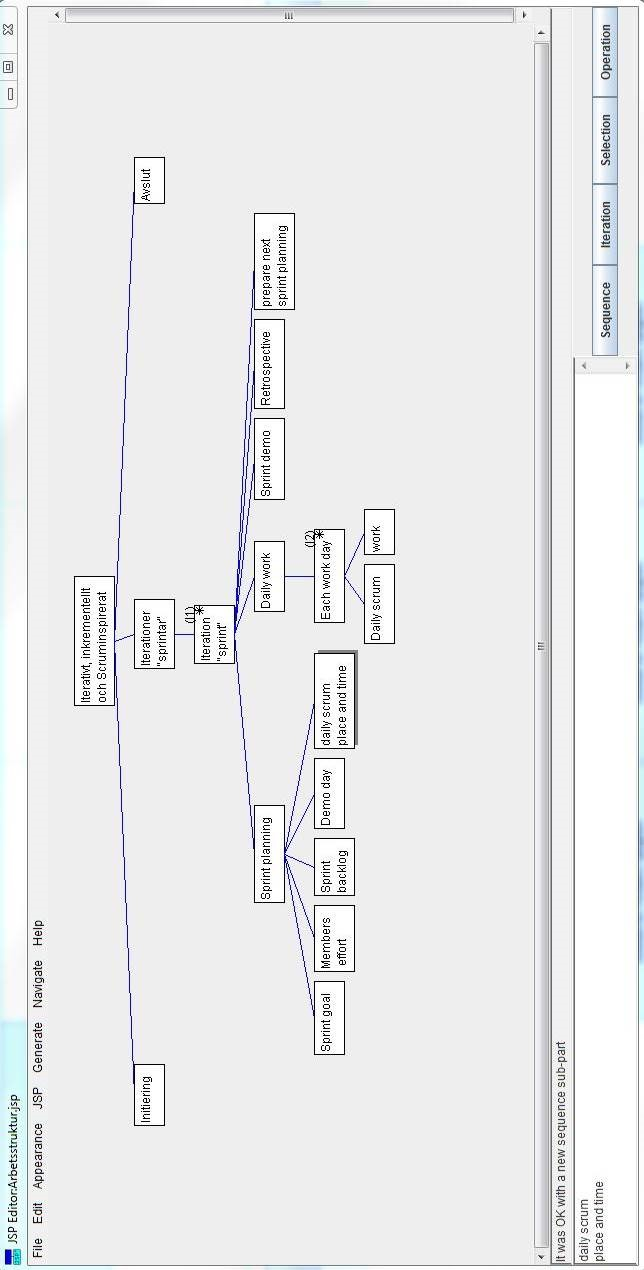
\includegraphics[max height=250px, max width=250px]{Z. images/scrum.jpg}}
        \caption{Den här har ingen beskrivning i mallen.}
        \label{fig}
    \end{figure}
\end{enumerate}